\documentclass{standalone}
\usepackage{tikz}
\usepackage{ctex,siunitx}
\setCJKmainfont{Noto Serif CJK SC}
\usepackage{tkz-euclide}
\usepackage{amsmath}
\usepackage{wasysym}
\usetikzlibrary{patterns, calc}
\usetikzlibrary {decorations.pathmorphing, decorations.pathreplacing, decorations.shapes,}
\begin{document}
\small
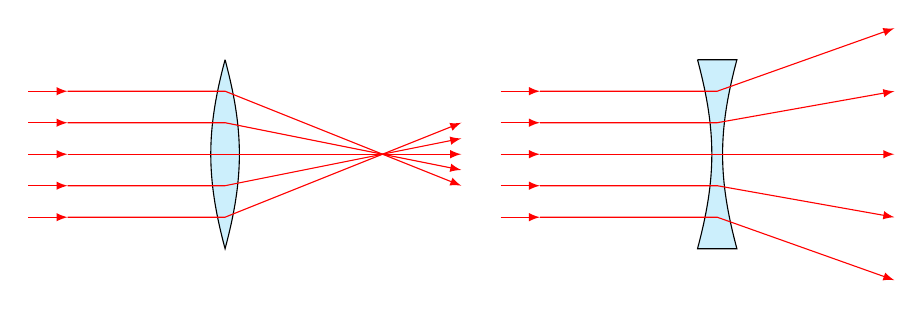
\begin{tikzpicture}[>=latex,scale=1.0]
  \draw [fill=cyan!20!white] (0,1.2) to [bend left=15] (0,-1.2) to [bend left=15](0,1.2);
  \foreach \x in {-.8,-.4,0,.4,.8}
  {
      \draw[red,->] (-2.5,\x)--(-2,\x);
      \draw[red,->] (-2,\x)--(0,\x)--(2,0)--(3,-0.5*\x);
  }    
  \begin{scope}[xshift=6cm]
    \draw [fill=cyan!20!white] (0,1.2) to [bend left=15] (0,-1.2)--(.5,-1.2) to [bend left=15](.5,1.2)--(0,1.2);
    \foreach \x in {-.8,-.4,0,.4,.8}
      {
          \draw[red,->] (-2.5,\x)--(-2,\x);
          \draw[red,->](-2,\x)--(0.25,\x)--(2.5,2*\x);
      }  
  \end{scope}
\end{tikzpicture}
\end{document}